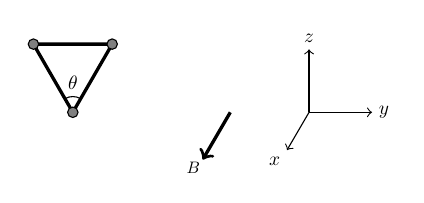
\begin{tikzpicture}
  \coordinate (H0) at (0, 0);
  \coordinate (H1) at ({sin(60/2)}, {cos(60/2)});
  \coordinate (H2) at ({-sin(60/2)}, {cos(60/2)});
  % =====================
  % Molecular arrangement
  % =====================
  \draw[very thick] (H1) -- (H0) -- (H2) -- cycle;
  \node[draw, shape=circle, fill=gray, scale=0.4] at (H0) {};
  \node[draw, shape=circle, fill=gray, scale=0.4] at (H1) {};
  \node[draw, shape=circle, fill=gray, scale=0.4] at (H2) {};
  \draw ({0.2*sin(60/2)}, {0.2*cos(60/2)}) arc [start angle=60, end angle=120, radius=0.2] node[anchor=south, midway, above, scale=.7] {$\theta$};
  % =====
  % Field
  % =====
  \draw[->, very thick] (2, 0) -- ++(-0.35, -0.6) node[scale=0.6, anchor=north east, inner sep=1pt] {$\symbfit{B}$};
  % =================
  % Coordinate system
  % =================
  \draw[->] (3, 0) -- ++(0.8, 0) node[anchor=west, scale=0.7] {$y$};
  \draw[->] (3, 0) -- ++(0, 0.8) node[anchor=south, scale=0.7] {$z$};
  \draw[->] (3, 0) -- ++(-0.28, -0.48) node[anchor=north east, scale=0.7] {$x$};
\end{tikzpicture}